% !TEX root = developer.tex

\newcommand{\nodecls}{\inlinecode{node}\xspace}
\newcommand{\topcls}{\inlinecode{topology}\xspace}
\newcommand{\switchid}{\inlinecode{switch_id}\xspace}
\newcommand{\nodeid}{\inlinecode{node_id}\xspace}

\chapter{Hardware Models}
\label{chapter:hardware}

\section{Overview}
\label{sec:topOverview}
To better understand how hardware models are put together for simulating interconnects, we should try to understand the basic flow of event in SST/macro involved in sending a message between two network endpoints.  We have already seen in skeleton applications in previous sections how an application-level call to a function like \inlinecode{MPI_Send} is mapping to an operating system function and finally a hardware-level injection of the message flow.  Overall, the following steps are required:

\begin{enumerate}
\item Start message flow with app-level function call
\item Push message onto NIC for send
\item NIC packetizes message and pushes packets on injection switch
\item Packets are routed and traverse the network
\item Packets arrive at destination NIC and are reassembled (potentially out-of-order)
\item Message flow is pushed up network software stack
\end{enumerate}

Through the network, packets must move through buffers (waiting for credits) and arbitrate for bandwidth through the switch crossbar and then through the ser/des link on the switch output buffers.  The control-flow diagram for transporting a flow from one endpoint to another via packets is shown in Figure \ref{fig:controlFlow}

\begin{figure}
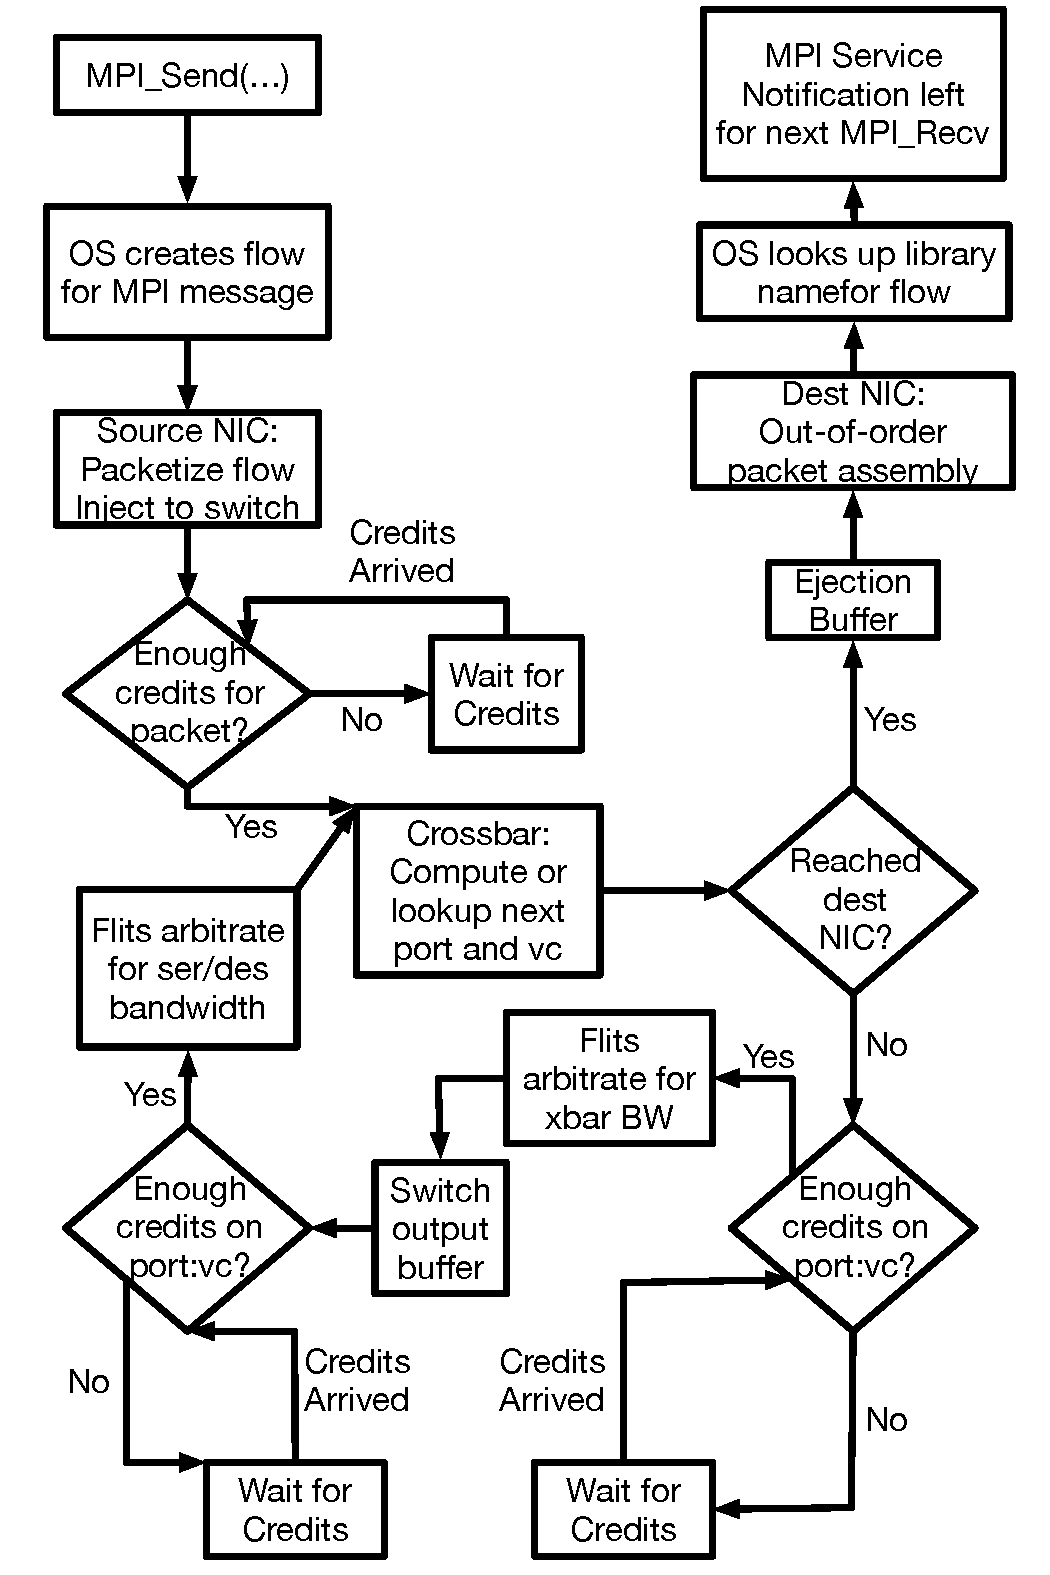
\includegraphics[width=0.8\textwidth]{figures/DecisionFlow}
\caption{Decision diagram showing the various control flow operations that occur as a message is transport across the network via individual packet operations.}
\label{fig:controlFlow}
\end{figure}

We can dive in deeper to the operations that occur on an individual component, mostly important the crossbar on the network switch. Figure \ref{fig:xbarFlow} shows code and program flow for a packet arriving at a network switch.  The packet is routed (virtual function, configurable via input file parameters), credits are allocated to the packet, and finally the packet is arbitrated across the crossbar. After arbitration, a statistics callback can be invoked to collect any performance metrics of interest (congestion, traffic, idle time).

\begin{figure}
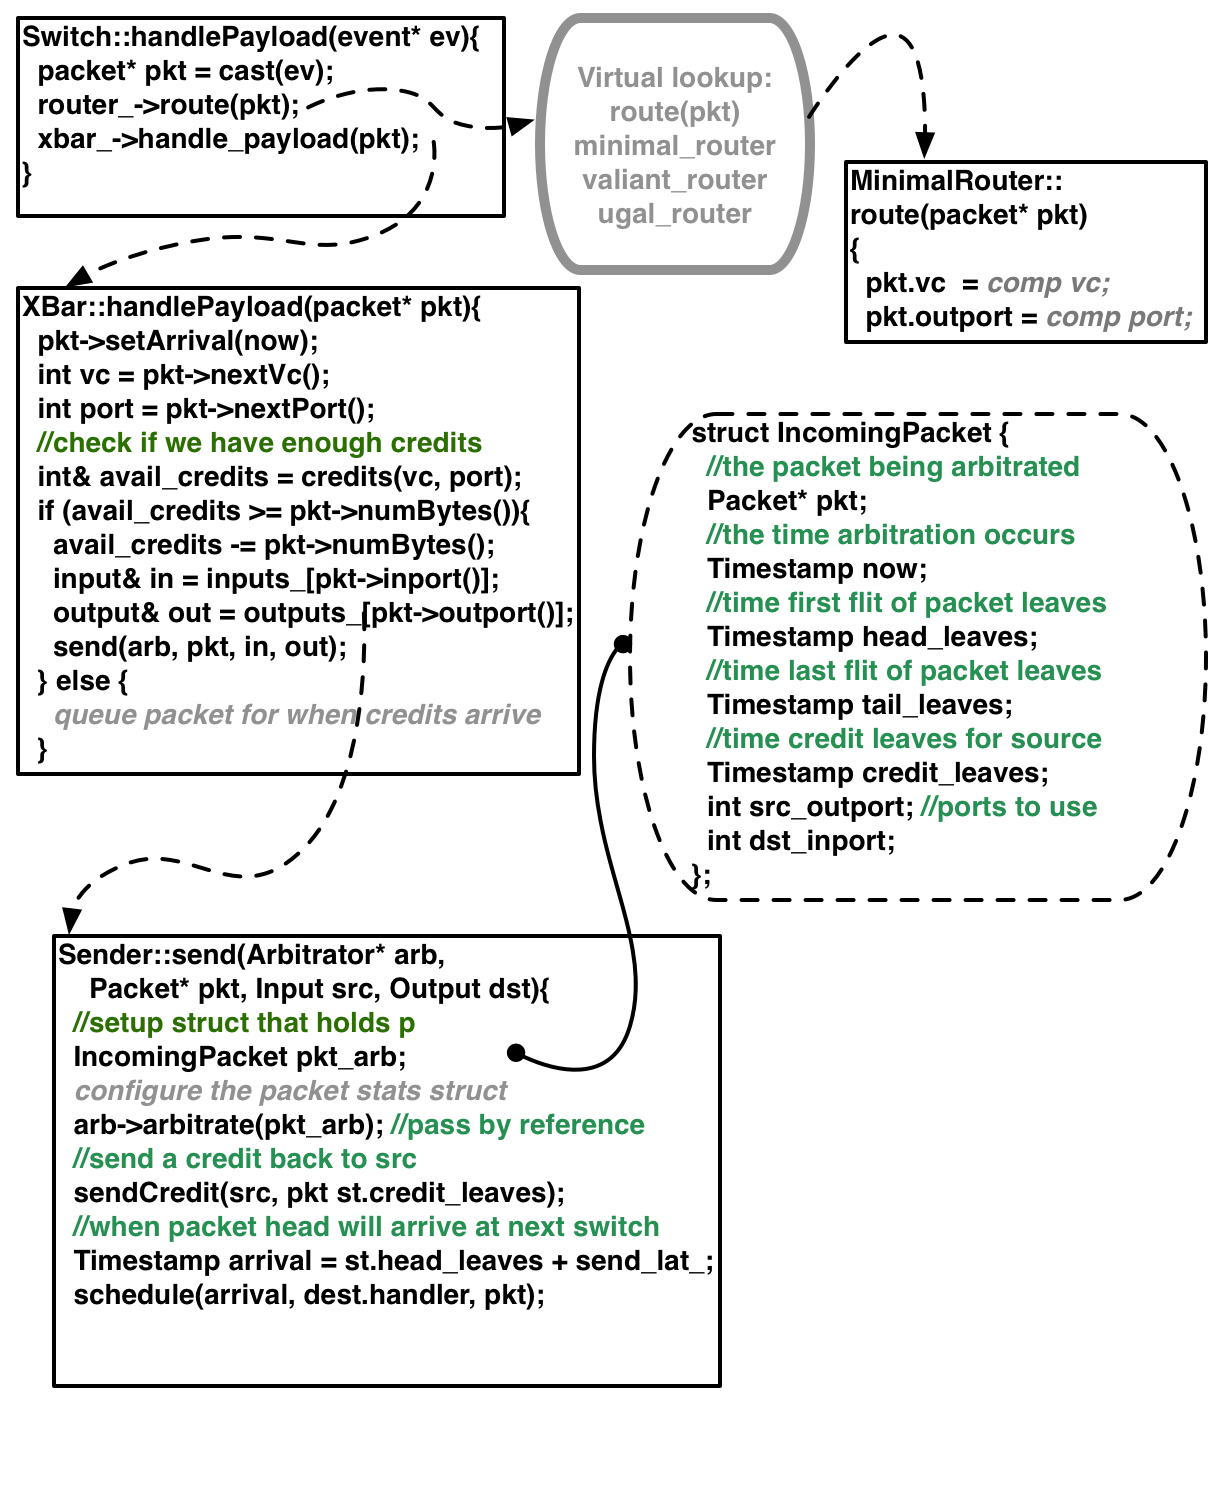
\includegraphics[width=0.9\textwidth]{figures/RoutingFlow}
\caption{Code flow for routing, arbitration, and stats collections of packets traversing the crossbar on the network switch.}
\label{fig:xbarFlow}
\end{figure}

\section{Connectables}
\label{sec:connectables}
With a basic overview of how the simulation proceeds, we can now look at the actual SST/macro class types.
While in common usage, \sstmacro follows a well-defined machine model (see below),
it generally allows any set of components to be connected. 
As discussed in Chapter \ref{chapter:des}, the simulation proceeds by having event components exchange messages,
each scheduled to arrive at a specific time.
\sstmacro provides a generic interface for any set of hardware components to be linked together.
Any hardware component that connects to other components and exchanges messages must inherit from the \inlinecode{connectable} class.
The \inlinecode{connectable} class presents a standard virtual interface

\begin{CppCode}
class connectable
{
 public:
  virtual void
  connect_output(
    sprockit::sim_parameters* params,
    int src_outport,
    int dst_inport,
    connectable* mod,
    event_handler* handler) = 0;

  virtual void
  connect_input(
    sprockit::sim_parameters* params,
    int src_outport,
    int dst_inport,
    connectable* mod,
    event_handler* handler) = 0;


};
\end{CppCode}

First, port numbers must be assigned identifying the output port at the source and in the input port at the destination.
For example, a switch may have several outgoing connections, each of which must be assigned a unique port number.
The connection must be configured at both source and destination.
The function is called twice for each side of the connection. If we have a source and destination:

\begin{CppCode}
connectable* src = ...
connectable* dst = ...
sprockit::sim_parameters* params = ...
src->connect_output(params, inport, outport, Output, dst);
dst->connect_input(params, inport, outport, Input, src);
\end{CppCode}

A certain style and set of rules is recommended for all connectables.
If these rules are ignored, setting up connections can quicky become confusing and produce difficult to maintain code.
The first and most important rule is that \inlinecode{connectables} never make their own connections.
Some ``meta''-object should create connections between objects.
In general, this work is left to a \inlinecode{interconnect} object.
An object should never be responsible for knowing about the ``world'' outside itself.
A topology or interconnect tells the object to make a connection rather than the object deciding to make the connection itself.
This will be illustrated below in \ref{sec:topology}.

The second rule to follow is that a connect function should never call another connect function.
In general, a single call to a connect function should create a single link.
If connect functions start calling other connect functions, you can end up a with a recursive mess.
If you need a bidirectional link (A $\rightarrow$ B, B $\rightarrow$ A),
two separate function calls should be made

\begin{CppCode}
A->connect_output(B);
B->connect_input(A);
\end{CppCode}

rather than having, e.g. A create a bidirectional link.

The first two rules should be considered rigorous. 
A third recommended rule is that all port numbers should be non-negative, and, in most cases, should start numbering from zero.


Combining the factory system for polymorphic types and the connectable system for building arbitrary machine links and topologies,
\sstmacro provides flexibility for building essentially any machine model you want.
However, \sstmacro provides a recommended machine structure to guide constructing machine models.

\section{Interconnect}\label{sec:topInterconnect}
For all standard runs, the entire hardware model is driven by the interconnect object.
The interconnect creates nodes, creates network switches, chooses a topology, and connects all of the network endpoints together.
In this regard, the interconnect also choose what types of components are being connected together.
For example, if you were going to introduce some custom FPGA device that connects to the nodes to perform filesystem operations,
the interconnect is responsible for creating it.

To illustrate, here is the code for the interconnect that creates the node objects. 
The interconnect is itself a factory object, configured from a parameter file.

\begin{CppCode}
interconnect::interconnect(sprockit::sim_parameters* params, event_manager* mgr, partition* part, parallel_runtime* rt)
{
  sprockit::sim_parameters* top_params = params->get_namespace("topology");
  topology_ = topology_factory::get_param("name", top_params);
  num_nodes_ = topology_->num_nodes();
  num_switches_ = topology_->num_switches();
  
  switches_.resize(num_switches_);
  nodes_.resize(num_nodes_);

  sprockit::sim_parameters* node_params = params->get_namespace("node");
  sprockit::sim_parameters* switch_params = params->get_namespace("switch");
  
  sprockit::sim_parameters* nic_params = node_params->get_namespace("nic");
  sprockit::sim_parameters* inj_params = nic_params->get_namespace("injection");
  sprockit::sim_parameters* ej_params = switch_params->get_namespace("ejection"); 
  
  build_endpoints(node_params, nic_params, mgr);
  build_switches(switch_params, mgr);
  connect_endpoints(inj_params, ej_params);
  connect_switches(switch_params); 
}
\end{CppCode}

For full details of the functions that build/connect endpoints and switches, consult the source code.
In general, the \inlinecode{interconnect} object uses the connectable interface to setup all the connections.
It uses the topology interface to determine which connections are required, e.g.

\begin{CppCode}
switch_id src = ...
std::vector<topology::connection> outports;
topology_->connected_outports(src, outports);
for (auto& conn : outports){
  network_switch* dst_sw = switches_[conn.dst];
  src_sw->connect_output(params, conn.src_outport, conn.dst_inport,
  					 dst_sw->payload_handler(conn.dst_inport));
  dst_sw->connect_input(params, conn.src_outport, conn.dst_inport,
  				       src_sw->credit_handler(conn.src_outport));
}
\end{CppCode}
The \inlinecode{connected_outports} function takes a given source switch and returns all the connections that the
switch is supposed to make.  Each switch must provide \inlinecode{payload_handler} and \inlinecode{ack_handler} functions to return
the \inlinecode{event_handler} that should receive either new packets (payload) or credits (ack) for the connections.

\section{Node}\label{sec:node}
Although the \nodecls can be implemented as a very complex model, it fundamentally only requires a single set of functions to meet the public interface.
The \nodecls must provide \inlinecode{execute_kernel} functions that are invoked by the \inlinecode{operating_system} or other other software objects.
The prototypes for these are:

\begin{CppCode}
virtual void
execute(ami::COMP_FUNC func, event* data);

virtual void
execute(ami::SERVICE_FUNC func, event* data);
\end{CppCode}	

By default, the abstract \nodecls class throws an \inlinecode{sprockit::unimplemented_error}. These functions are not pure virtual.
A node is only required to implement those functions that it needs to do.
The various function parameters are enums for the different operations a node may perform:
computation or communication. Computation functions are those that require compute resources. Service functions are special functions that run in the background and ``lightweight'' such that any modeling of processor allocation should be avoided. Service functions are run ``for free'' with no compute 

\section{Network Interface (NIC)}\label{sec:nic}
The network interface can implement many services, but the basic public interface requires the NIC to do three things:

\begin{itemize}
\item Inject messages into the network
\item Receive messages ejected from the network
\item Deliver ACKs (acknowledgments) of message delivery
\end{itemize}

For sending messages, the NIC must implement

\begin{CppCode}
  virtual void
  do_send(network_message* payload);
\end{CppCode}
A non-virtual, top-level \inlinecode{send} function performs operations standard to all NICs.
Once these operations are complete, the NIC invokes \inlinecode{do_send} to perform model-specific send operations.
The NIC should only ever send \inlinecode{network_message} types.

For the bare-bones class \inlinecode{logp_nic}, the function is

\begin{CppCode}
void
logp_nic::do_send(network_message* msg)
{
  long num_bytes = msg->byte_length();
  timestamp now_ = now();
  timestamp start_send = now_ > next_free_ ? now_ : next_free_;
  timestamp time_to_inject = inj_lat_ + timestamp(inj_bw_inverse_ * num_bytes);
  //leave the injection latency term to the interconnect
  schedule_now(injection_switch_, msg);

  next_free_ = start_send + time_to_inject;
  if (msg->needs_ack()) {
    //do whatever you need to do so that this msg decouples all pointers
    network_message* acker = msg->clone_injection_ack();
    schedule(next_free_, parent_->self_handler(), acker); //send to node
  }
}
\end{CppCode}
After injecting, the NIC creates an ACK and delivers the notification to the \nodecls.
In general, all arriving messages or ACKs should be delivered to the node.
The node is responsible for generating any software events in the OS.

For receiving, messages can be moved across the network and delivered in two different ways:
either at the byte-transfer layer (BTL) or message-transfer layer (MTL).
Depending on the congestion model, a large message (say a 1 MB MPI message) might be broken up into many packets.
These message chunks are moved across the network independently and then reassembled at the receiving end.
Alternatively, for flow models or simple analytical models, the message is not packetized and instead delivered as a single whole.
The methods are not pure virtual.  Depending on the congestion model,  the NIC might only implement chunk receives or whole receives.
Upon receipt, just as for ACKs, the NIC should deliver the message to the node to interpret.
In general, \inlinecode{nic::handle} is intended to handle packets. 
If a NIC supports direct handling of complete messages (MTL) instead of packets (BTL),
it should provide a message handler:

\begin{CppCode}
event_handler*
mtl_handler() const {
  return mtl_handler_;
}
\end{CppCode}

A special completion queue object tracks chunks and processes out-of-order arrivals,
notifying the NIC when the entire message is done.

\section{Memory Model}\label{sec:memModel}
As with the NIC and node, the memory model class can have a complex implementation under the hood,
but it must funnel things through the a common function.

\begin{CppCode}
virtual void
access(long bytes, double max_bw) = 0;
\end{CppCode}

This function is intended to be called from an application user-space thread.
As such, it should block until complete.
For more details on the use of user-space threading to model applications,
see the User's manual.


\section{Network Switch}\label{sec:networkSwitch}

Unlike the other classes above, a network switch is not required to implement any specific functions.
It is only required to be an \inlinecode{event_handler}, providing the usual \inlinecode{handle(event* ev)}.
The internal details can essentially be arbitrary.
However, the basic scheme for most switches follows the code below for the \inlinecode{pisces} model.

\begin{CppCode}
void
pisces_switch::handle_credit(event *ev)
{
  pisces_credit* credit = static_cast<pisces_credit*>(ev);
  out_buffers_[credit->port()]->handle_credit(credit);
}

void
pisces_switch::handle_payload(event *ev)
{
  pisces_payload* payload = static_cast<pisces_payload*>(ev);
  router_->route(payload);
  xbar_->handle_payload(payload);
}
\end{CppCode}
The arriving event is sent to either a credit handler or a payload handler,
which is configured during simulation setup.
If a packet, the router object selects the next destination (port).
The packet is then passed to the crossbar for arbitration.

\section{Topology}
\label{sec:topology}
Of critical importance for the network modeling is the topology of the interconnect.
Common examples are the torus, fat tree, or butterfly.
To understand what these topologies are, there are many resources on the web.
Regardless of the actual structure as a torus or tree, the topology should present a common interface to the interconnect and NIC for routing messages.
Here we detail the public interface.

\subsection{Basic Topology}
\label{subsec:basicTopology}
Not all topologies are ``regular'' like a torus.  Ad hoc computer networks (like the internet) are ordered with IP addresses, but don't follow a regular geometric structure.
The abstract topology base class is intended to cover both cases.
Irregular or arbitrary topology connections are not fully supported yet.

The most important functions in the \topcls class are

\begin{CppCode}
class topology
{
virtual bool
uniform_network_ports() const = 0;

virtual bool
uniform_switches_non_uniform_network_ports() const = 0;

virtual bool
uniform_switches() const = 0;

virtual void
connected_outports(switch_id src, std::vector<topology::connection>& conns) const = 0;

virtual void
configure_individual_port_params(switch_id src,
      sprockit::sim_parameters* switch_params) const = 0;

virtual int
num_switches() const = 0;

virtual int
num_leaf_switches() const = 0;

virtual int
num_nodes() const = 0;

virtual int
num_endpoints() const = 0;

virtual int
max_num_ports() const = 0;

virtual switch_id
netlink_to_injection_switch(node_id nodeaddr, int& switch_port) const = 0;

virtual switch_id
netlink_to_ejection_switch(node_id nodeaddr, int& switch_port) const = 0;

virtual void
configure_vc_routing(std::map<routing::algorithm_t, int>& m) const = 0;

virtual switch_id
node_to_ejection_switch(node_id addr, int& port) const = 0;

virtual int
minimal_distance(switch_id src, switch_id dst) const = 0;

virtual int
num_hops_to_node(node_id src, node_id dst) const = 0;

virtual void
nodes_connected_to_injection_switch(switch_id swid,
                      std::vector<injection_port>& nodes) const = 0;

virtual void
nodes_connected_to_ejection_switch(switch_id swid,
                      std::vector<injection_port>& nodes) const = 0;

virtual void
minimal_route_to_switch(
switch_id current_sw_addr,
switch_id dest_sw_addr,
routable::path& path) const = 0;

virtual bool
node_to_netlink(node_id nid, node_id& net_id, int& offset) const = 0;
\end{CppCode}

These functions are documented in the \inlineshell{topology.h} header file.
The first few functions just give the number of switches, number of nodes, and finally which nodes are connected to a given switch.
Each compute node will be connected to an injector switch and an ejector switch (often the same switch).
The topology must provide a mapping between a node and its ejection and injection points.
Additionally, the topology must indicate a port number or offset for the injection in case the switch has many nodes injecting to it.
The most important thing to distinguish here are \nodeid and \switchid types.
These are typedefs that distinguish between a switch in the topology and a node or network endpoint.

Besides just forming the connections, a topology is responsible for routing.
Given a source switch and the final destination, a topology must fill out path information.

\begin{CppCode}
struct path {
    int outport;
    int vc;
    int geometric_id;
    sprockit::metadata_bits<uint32_t> metadata;
}
\end{CppCode}

The most important information is the outport, telling a switch which port to route along to arrive at the destination.
For congestion models with channel dependencies, the virtual channel must also be given to avoid deadlock.
In general, network switches and other devices should be completely topology-agnostic.
The switch is responsible for modeling congestion within itself - crossbar arbitration, credits, outport multiplexing.
The switch is not able to determine for itself which outport to route along.
The topology tells the switch which port it needs and the switch determines what sort of congestion delay to expect on that port.
This division of labor is complicated a bit by adaptive routing, but remains essentially the same.  More details are given later.

\section{Router}\label{sec:router}
The router has a simple public interface

\begin{CppCode}
class router
{
...
  virtual void
  route(packet* pkt);

  virtual void
  route_to_switch(switch_id sid, routable::path& path) = 0;
...
};
\end{CppCode}

Different routers exist for the different routing algorithms: 	minimal, valiant, ugal.
The router objects are specific to a switch and can therefore store state information.
However, the router should query the topology object for any path-specific information, e.g.

\begin{CppCode}
void
minimal_router::route_to_switch(switch_id sid, routable::path& path)
{
  top_->minimal_route_to_switch(my_addr_, sid, path);
}
\end{CppCode}

For adaptive routing, a bit more work is done.
Each router is connect to a switch object which holds all the information about queue lengths, e.g.

\begin{CppCode}
int test_length = get_switch()->queue_length(paths[i].outport);
\end{CppCode}
allowing the router to select an alternate path if the congestion is too high. 


